\documentclass{../../slides-style}

\slidetitle{Об архитектуре программного обеспечения}{20.05.2025}

\begin{document}

    \begin{frame}[plain]
        \titlepage
    \end{frame}

    \section{Профессия \enquote{Архитектор}}

    \begin{frame}
        \frametitle{Архитектура}
        \begin{columns}
            \begin{column}{0.7\textwidth}
                \begin{itemize}
                    \item Совокупность важнейших решений об организации программной системы
                    \begin{itemize}
                        \item Эволюционирующий свод знаний
                        \item Разные точки зрения
                        \item Разный уровень детализации
                    \end{itemize}
                    \item Для чего
                    \begin{itemize}
                        \item База для реализации, \enquote{фундамент} системы
                        \item Инструмент для оценки трудоёмкости и отслеживания прогресса
                        \item Средство обеспечения переиспользования
                        \item Средство анализа системы ещё до того, как она реализована
                    \end{itemize}
                \end{itemize}
            \end{column}
            \begin{column}{0.3\textwidth}
                \begin{center}
                    \includegraphics[width=\textwidth]{whatArchitecture.png}
                \end{center}
                \attribution{Интернеты}
            \end{column}
        \end{columns}
    \end{frame}

    \begin{frame}
        \frametitle{Профессия \enquote{Архитектор}}
        \begin{itemize}
            \item Архитектор --- человек (или группа людей), отвечающий за:
            \begin{itemize}
                \item разработку и описание архитектуры системы
                \item доведение её до всех заинтересованных лиц
                \item контроль реализации архитектуры
                \item поддержание её актуального состояния по ходу разработки и сопровождения
            \end{itemize}
        \end{itemize}
    \end{frame}

    \begin{frame}
        \frametitle{Архитектор vs разработчик}
        \begin{center}
            \includegraphics[width=0.35\textwidth]{architectVsDeveloper.png}
        \end{center}
        \begin{itemize}
            \item Широта знаний
            \item Коммуникационные навыки
            \item Часто архитектор играет роль разработчика и наоборот
        \end{itemize}
    \end{frame}

    \section{Моделирование}

    \begin{frame}
        \frametitle{Моделирование ПО}
        \begin{itemize}
            \item Основной продукт архитектора --- архитектурная документация
            \item Модели --- важная её часть
            \begin{itemize}
                \item Предназначены прежде всего для управления сложностью
                \item Могут моделировать как саму систему, так и окружение
                \item Позволяют понять, проанализировать и протестировать систему до её реализации
            \end{itemize}
        \end{itemize}
        \begin{center}
            \includegraphics[width=0.3\textwidth]{vendingMachine.png}
            \attribution{N. Medvidovic}
        \end{center}
    \end{frame}

    \begin{frame}
        \frametitle{Unified Modeling Language}
        \begin{itemize}
            \item Семейство графических нотаций
            \begin{itemize}
                \item 14 видов диаграмм
            \end{itemize}
            \item Общая метамодель
            \item Стандарт под управлением Object Management Group
            \begin{itemize}
                \item UML 1.1 --- 1997 год
                \item UML 2.0 --- 2005 год
                \item UML 2.5.1 --- декабрь 2017 года
            \end{itemize}
            \item Прежде всего, для проектирования ПО
            \begin{itemize}
                \item После UML 2.0 стали появляться нотации и для инженеров
            \end{itemize}
            \item Расширяем, но сложно
        \end{itemize}
    \end{frame}

    \begin{frame}
        \frametitle{Виды диаграмм}
        \begin{center}
            \includegraphics[width=\textwidth]{umlDiagrams.png}
        \end{center}
    \end{frame}

    \begin{frame}
        \frametitle{Диаграмма классов}
        \begin{center}
            \includegraphics[height=0.8\textheight]{umlClassDiagram.png}
            \attribution{М. Фаулер. \enquote{UML. Основы}}
        \end{center}
    \end{frame}

    \begin{frame}
        \frametitle{Диаграмма компонентов}
        \begin{center}
            \includegraphics[width=0.95\textwidth]{componentDiagrams.png}
        \end{center}
    \end{frame}

    \begin{frame}
        \frametitle{Диаграмма случаев использования UML}
        \framesubtitle{Диаграмма прецедентов}
        \begin{columns}
            \begin{column}{0.5\textwidth}
                \begin{itemize}
                    \item Ивар Якобсон, 1992 год
                    \item Акторы (или актёры, роли) --- внешние сущности, использующие систему
                    \begin{itemize}
                        \item Люди или другие программные системы
                    \end{itemize}
                    \item Случаи использования (прецеденты)  --- цель использования системы актором
                    \begin{itemize}
                        \item Раскрываются в набор сценариев, описываемых чаще текстом
                    \end{itemize}
                \end{itemize}
            \end{column}
            \begin{column}{0.5\textwidth}
                \begin{center}
                    \includegraphics[width=\textwidth]{useCaseDiagram.png}
                    \attribution{М. Фаулер, UML. Основы}
                \end{center}
            \end{column}
        \end{columns}
    \end{frame}

    \begin{frame}
        \frametitle{Диаграмма активностей UML}
        \framesubtitle{Диаграммы деятельности}
        \begin{columns}
            \begin{column}{0.5\textwidth}
                \begin{itemize}
                    \item Используются для моделирования бизнес-процессов, тоже на первых этапах
                    \begin{itemize}
                        \item Может быть визуализацией сценария использования
                    \end{itemize}
                    \item Иногда --- для моделирования алгоритма
                    \item Расширенные блок-схемы
                \end{itemize}
            \end{column}
            \begin{column}{0.5\textwidth}
                \begin{center}
                    \includegraphics[width=0.7\textwidth]{activityDiagram.png}
                    \attribution{М. Фаулер, UML. Основы}
                \end{center}
            \end{column}
        \end{columns}
    \end{frame}

    \begin{frame}
        \frametitle{Инструменты для рисования диаграмм}
        \begin{itemize}
            \item \enquote{Рисовалки}
            \begin{itemize}
                \item \url{https://diagrams.net/}
                \item Visio
                \item Dia
                \item SmartDraw
                \item LucidChart
                \item \url{http://plantuml.com/}
            \end{itemize}
            \item Полноценные CASE-системы
            \begin{itemize}
                \item Visual Paradigm
                \item Enterprise Architect
                \item Rational Software Architect
                \item MagicDraw
            \end{itemize}
            \item Браузерные инструменты
            \begin{itemize}
                \item \url{https://www.websequencediagrams.com/}
                \item \url{http://yuml.me/}
            \end{itemize}
        \end{itemize}
    \end{frame}

    \section{Базовые принципы хорошего дизайна}

    \subsection{Принципы SOLID}

    \begin{frame}
        \frametitle{Принципы SOLID}
        \begin{itemize}
            \item Single responsibility principle
            \item Open/closed principle
            \item Liskov substitution principle
            \item Interface segregation principle
            \item Dependency inversion principle
        \end{itemize}
    \end{frame}

    \begin{frame}
        \frametitle{Single responsibility principle}
        \begin{itemize}
            \item Каждый объект должен иметь одну обязанность
            \item Эта обязанность должна быть полностью инкапсулирована в объект
        \end{itemize}
        \begin{flushright}
            \includegraphics[width=0.25\textwidth]{singleResponsibility.png}
        \end{flushright}
    \end{frame}

    \begin{frame}
        \frametitle{Open/closed principle}
        \begin{itemize}
            \item Программные сущности (классы, модули, функции и т. п.) должны быть открыты для расширения, но закрыты для изменения
            \begin{itemize}
                \item Переиспользование через наследование
                \item Неизменные интерфейсы
            \end{itemize}
        \end{itemize}
        \begin{flushright}
            \includegraphics[width=0.5\textwidth]{openClosedPrinciple.png}
        \end{flushright}
    \end{frame}

    \begin{frame}
        \frametitle{Liskov substitution principle}
        \begin{itemize}
            \item Функции, которые используют базовый тип, должны иметь возможность использовать подтипы базового типа, не зная об этом
        \end{itemize}
        \begin{flushright}
            \includegraphics[width=0.4\textwidth]{liskovSubstitutionPrinciple.png}
        \end{flushright}
    \end{frame}

    \begin{frame}
        \frametitle{Interface segregation principle}
        \begin{itemize}
            \item Клиенты не должны зависеть от методов, которые они не используют
            \begin{itemize}
                \item Слишком \enquote{толстые} интерфейсы необходимо разделять на более мелкие и специфические
            \end{itemize}
        \end{itemize}
        \begin{flushright}
            \includegraphics[width=0.5\textwidth]{interfaceSegregationPrinciple.png}
        \end{flushright}
    \end{frame}

    \begin{frame}
        \frametitle{Dependency inversion principle}
        \begin{itemize}
            \item Модули верхних уровней не должны зависеть от модулей нижних уровней. Оба типа модулей должны зависеть от абстракций
            \item Абстракции не должны зависеть от деталей. Детали должны зависеть от абстракций
        \end{itemize}
        \begin{flushright}
            \includegraphics[width=0.5\textwidth]{dependencyInversionPrinciple.png}
        \end{flushright}
    \end{frame}

    \subsection{Закон Деметры}

    \begin{frame}
        \frametitle{Закон Деметры}
        \begin{itemize}
            \item \enquote{Не разговаривай с незнакомцами!}
            \item Объект A не должен иметь возможность получить непосредственный доступ к объекту C, если у объекта A есть доступ к объекту B, и у объекта B есть доступ к объекту C
            \item \mintinline{java}|book.pages().last().text()| vs \mintinline{java}|book.lastPageText()|
            \item Иногда называют \enquote{Крушение поезда}
        \end{itemize}
        \begin{flushright}
            \includegraphics[width=0.35\textwidth]{trains.png}
        \end{flushright}
        \vspace{-0.8cm}
        \attribution{Р. Мартин, \enquote{Чистый код}}
    \end{frame}

    \subsection{Другие принципы}

    \begin{frame}
        \frametitle{Другие принципы}
        \begin{itemize}
            \item Don't Repeat Yourself (DRY), он же \enquote{Копипаст суть ересь}
            \item Keep It Simple, Stupid (KISS)
            \item You Aren't Gonna Need It (YAGNI), он же \enquote{нет Big Design Up Front}
        \end{itemize}
    \end{frame}

    \section{Паттерны проектирования}

    \begin{frame}
        \frametitle{Паттерны проектирования}
        \textbf{Шаблон проектирования} --- это повторимая архитектурная конструкция, являющаяся решением некоторой типичной технической проблемы
        \begin{itemize}
            \item Подходит для класса проблем
            \item Обеспечивает переиспользуемость знаний
            \item Позволяет унифицировать терминологию
            \item В удобной для изучения форме
            \item НЕ конкретный рецепт или указания к действию
        \end{itemize}
    \end{frame}

    \subsection{Паттерн \enquote{Стратегия}}

    \begin{frame}
        \frametitle{Форматирование текста}
        \begin{itemize}
            \item Задача --- разбиение текста на строки, колонки и т.д.
            \item Высокоуровневые параметры форматирования
            \begin{itemize}
                \item Ширина полей, размер отступа, межстрочный интервал и т.д.
            \end{itemize}
            \item Компромисс между качеством и скоростью работы
            \item Инкапсуляция алгоритма
        \end{itemize}
    \end{frame}

    \begin{frame}
        \frametitle{Compositor и Composition}
        \begin{center}
            \includegraphics[width=0.7\textwidth]{compositor.png}
            \attribution{Э. Гамма и др., Приемы объектно-ориентированного проектирования}
        \end{center}
    \end{frame}

    \begin{frame}
        \frametitle{Паттерн \enquote{Стратегия}}
        \framesubtitle{Strategy}
        \begin{itemize}
            \item Назначение --- инкапсуляция алгоритма в объект
            \item Самое важное --- спроектировать интерфейсы стратегии и контекста
            \begin{itemize}
                \item Так, чтобы не менять их для каждой стратегии
            \end{itemize}
            \item Применяется, если
            \begin{itemize}
                \item Имеется много родственных классов с разным поведением
                \item Нужно иметь несколько вариантов алгоритма
                \item В алгоритме есть данные, про которые клиенту знать не надо
                \item В коде много условных операторов
            \end{itemize}
        \end{itemize}
        \begin{center}
            \includegraphics[width=0.6\textwidth]{strategy.png}
        \end{center}
    \end{frame}

    \begin{frame}
        \frametitle{\enquote{Стратегия} (Strategy), детали реализации}
        \begin{center}
            \includegraphics[width=0.6\textwidth]{strategy.png}
        \end{center}
        \begin{itemize}
            \item Передача контекста вычислений в стратегию
            \begin{itemize}
                \item Как параметры метода --- уменьшает связность, но некоторые параметры могут быть стратегии не нужны
                \item Передавать сам контекст в качестве аргумента --- в Context интерфейс для доступа к данным
            \end{itemize}
            \item Стратегия может быть параметром шаблона
            \begin{itemize}
                \item Если не надо её менять на лету
                \item Не надо абстрактного класса и нет оверхеда на вызов виртуальных методов
            \end{itemize}
            \item Стратегия по умолчанию
        \end{itemize}
    \end{frame}

    \section{Что почитать}

    \begin{frame}
        \frametitle{Что почитать}
        \begin{columns}
            \begin{column}{0.6\textwidth}
                \begin{itemize}
                    \item Э. Гамма, Р. Хелм, Р. Джонсон, Дж. Влиссидес, Приемы объектно-ориентированного проектирования. Паттерны проектирования.
                    \item Мартин Фаулер, UML: основы.
                    \item Роберт Мартин, Чистый код: создание, анализ и рефакторинг
                \end{itemize}
            \end{column}
            \begin{column}{0.4\textwidth}
                \begin{center}
                    \includegraphics[width=0.8\textwidth]{patternBookCover.png}
                \end{center}
            \end{column}
        \end{columns}
    \end{frame}

\end{document}